% -----------------------------------------------------------------------------
% Copyright © Institut National de la Recherche Scientifique (INRS)
% https://github.com/cgq-qgc/rsesq-bulletin
%
% Created by Jean-Sébastien Gosselin
% jean-sebastien.gosselin@inrs.ca
%
% This work is licensed under the terms of the CC BY 4.0 License as published
% by the Creative Commons nonprofit organization. For more details, see the
% CC BY 4.0 License at https://creativecommons.org/licenses/by/4.0/.
% -----------------------------------------------------------------------------

% Fonction de réponse barométrique (FRB)

\newpage
\noindent
\begin{tcbposter}[
poster = {
  % showframe,
  columns = 1,
  rows = 2,
  height= \textheight,
  width = \textwidth},
boxes = {
  colback=white, colframe=white, coltitle=blue, arc=0pt}
]
\posterbox[adjusted title=Fonction de réponse barométrique (FRB)\\,
           valign=center, halign=center, center title, left*=0pt, right*=0pt,
           bottom=0pt, boxsep=0pt, colframe=white,
           fonttitle=\subtitlefont]
  {name=brfgraph, row=1, column=1, below=top}
  {\includegraphics[width=0.85\linewidth]{\pathbrf}}
\posterbox[adjusted title=Éléments de théorie, boxrule=\boxrule,
           colframe=blue,
           fonttitle=\boxtitlefont,
%           parbox=false
           sidebyside,righthand width=8cm, lower separated=false,
           before upper={\parindent15pt\noindent}
           ]
  {name=brftheory, row=2, column=1, above=bottom}
  {
  Les variations de la pression atmosphérique sont connues pour causer des 
  fluctuations proportionnelles et opposées du niveau d'eau dans les puits.
  La réponse temporelle du niveau d'eau aux variations de la pression 
  atmosphérique peut être caractérisée par une équation mathématique que l'on
  nomme la fonction de réponse barométrique (FRB).

  \indent L'allure de la courbe de la FRB est caractéristique des propriétés 
  hydrauliques et géométriques du puits, de même que des propriétés mécaniques 
  et du niveau de confinement de l'aquifère dans lequel le puits est installé. 
  La comparaison de la FRB calculée pour un puits donné aux courbes 
  théoriques (voir figure ci-contre) permet entre autres de renseigner sur le 
  niveau de confinement et la transmissivité de l'aquifère dans 
  l'environnement du puits.
  \tcblower
  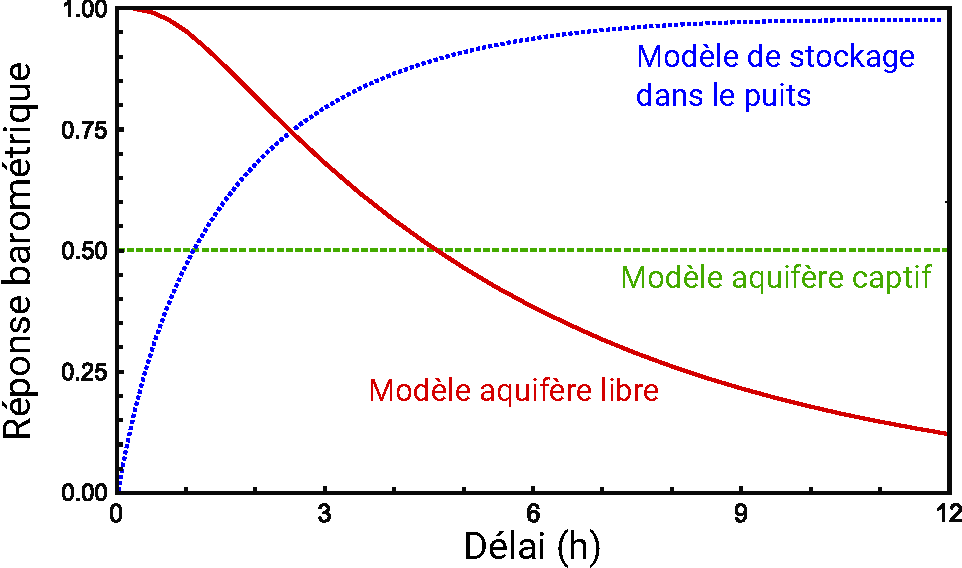
\includegraphics[width=\linewidth]{D113 Spane_2002.pdf}
  }
\end{tcbposter}
